\subsection{Mediator Pattern}


\subsubsection*{Problembeschreibung}

Große Softwareprojekte bestehen meist aus einer einer enormen Anzahl an Klassen bzw. Objekten, welche miteinander interagieren. Ziel ist es stets, die Kopplung zwischen diesen Komponenten so gering wie möglich zu halten. Komplexe Interaktionsmuster zwischen diesen Objekten lassen sich nicht immer verhindern, das sie die inhärente Komplexität des modellierten Problems wiederspiegeln. In diesem Fall ist eine Lösung notwending, die diese Komplexität kapselt. Das Mediator-Pattern ist in der Lage, solche Fälle von komplexer Interaktion zu vereinfachen.

\subsubsection*{Lösung}

Der konkrete Mediator implementiert das Mediator-Interface, welches eine Methode `notify` bereitstellt, um Benachrichtigungen der einzelnen Komponenten entgegenzunehmen. Jede Komponente besitzt eine Referenz auf den Mediator, um `notify`an ihn senden zu können. Dabei übergibt die Komponente sich selbst, um dem Mediator den Kontext der Benachrichtigung bereitzustellen. In Abhängigkeit des übergebenen Senders und dessen Zustand, führt der Mediator eine (komplexe) Logik aus, welche vollständig innerhalb des Mediators gekapselt ist. Der Mediator hält ebenso Referenzen auf alle Komponenten, die er zu beeinflussen in der Lage sein soll. Die gekapselte Logik kann somit die Interfaces der Komponenten verwenden, um diese zu beeinflussen. Dadurch findet eine indirekte Beeinflussung von Komponenten durch andere Komponenten über den Mediator statt.  

\begin{figure}[!hb]
	\centering
	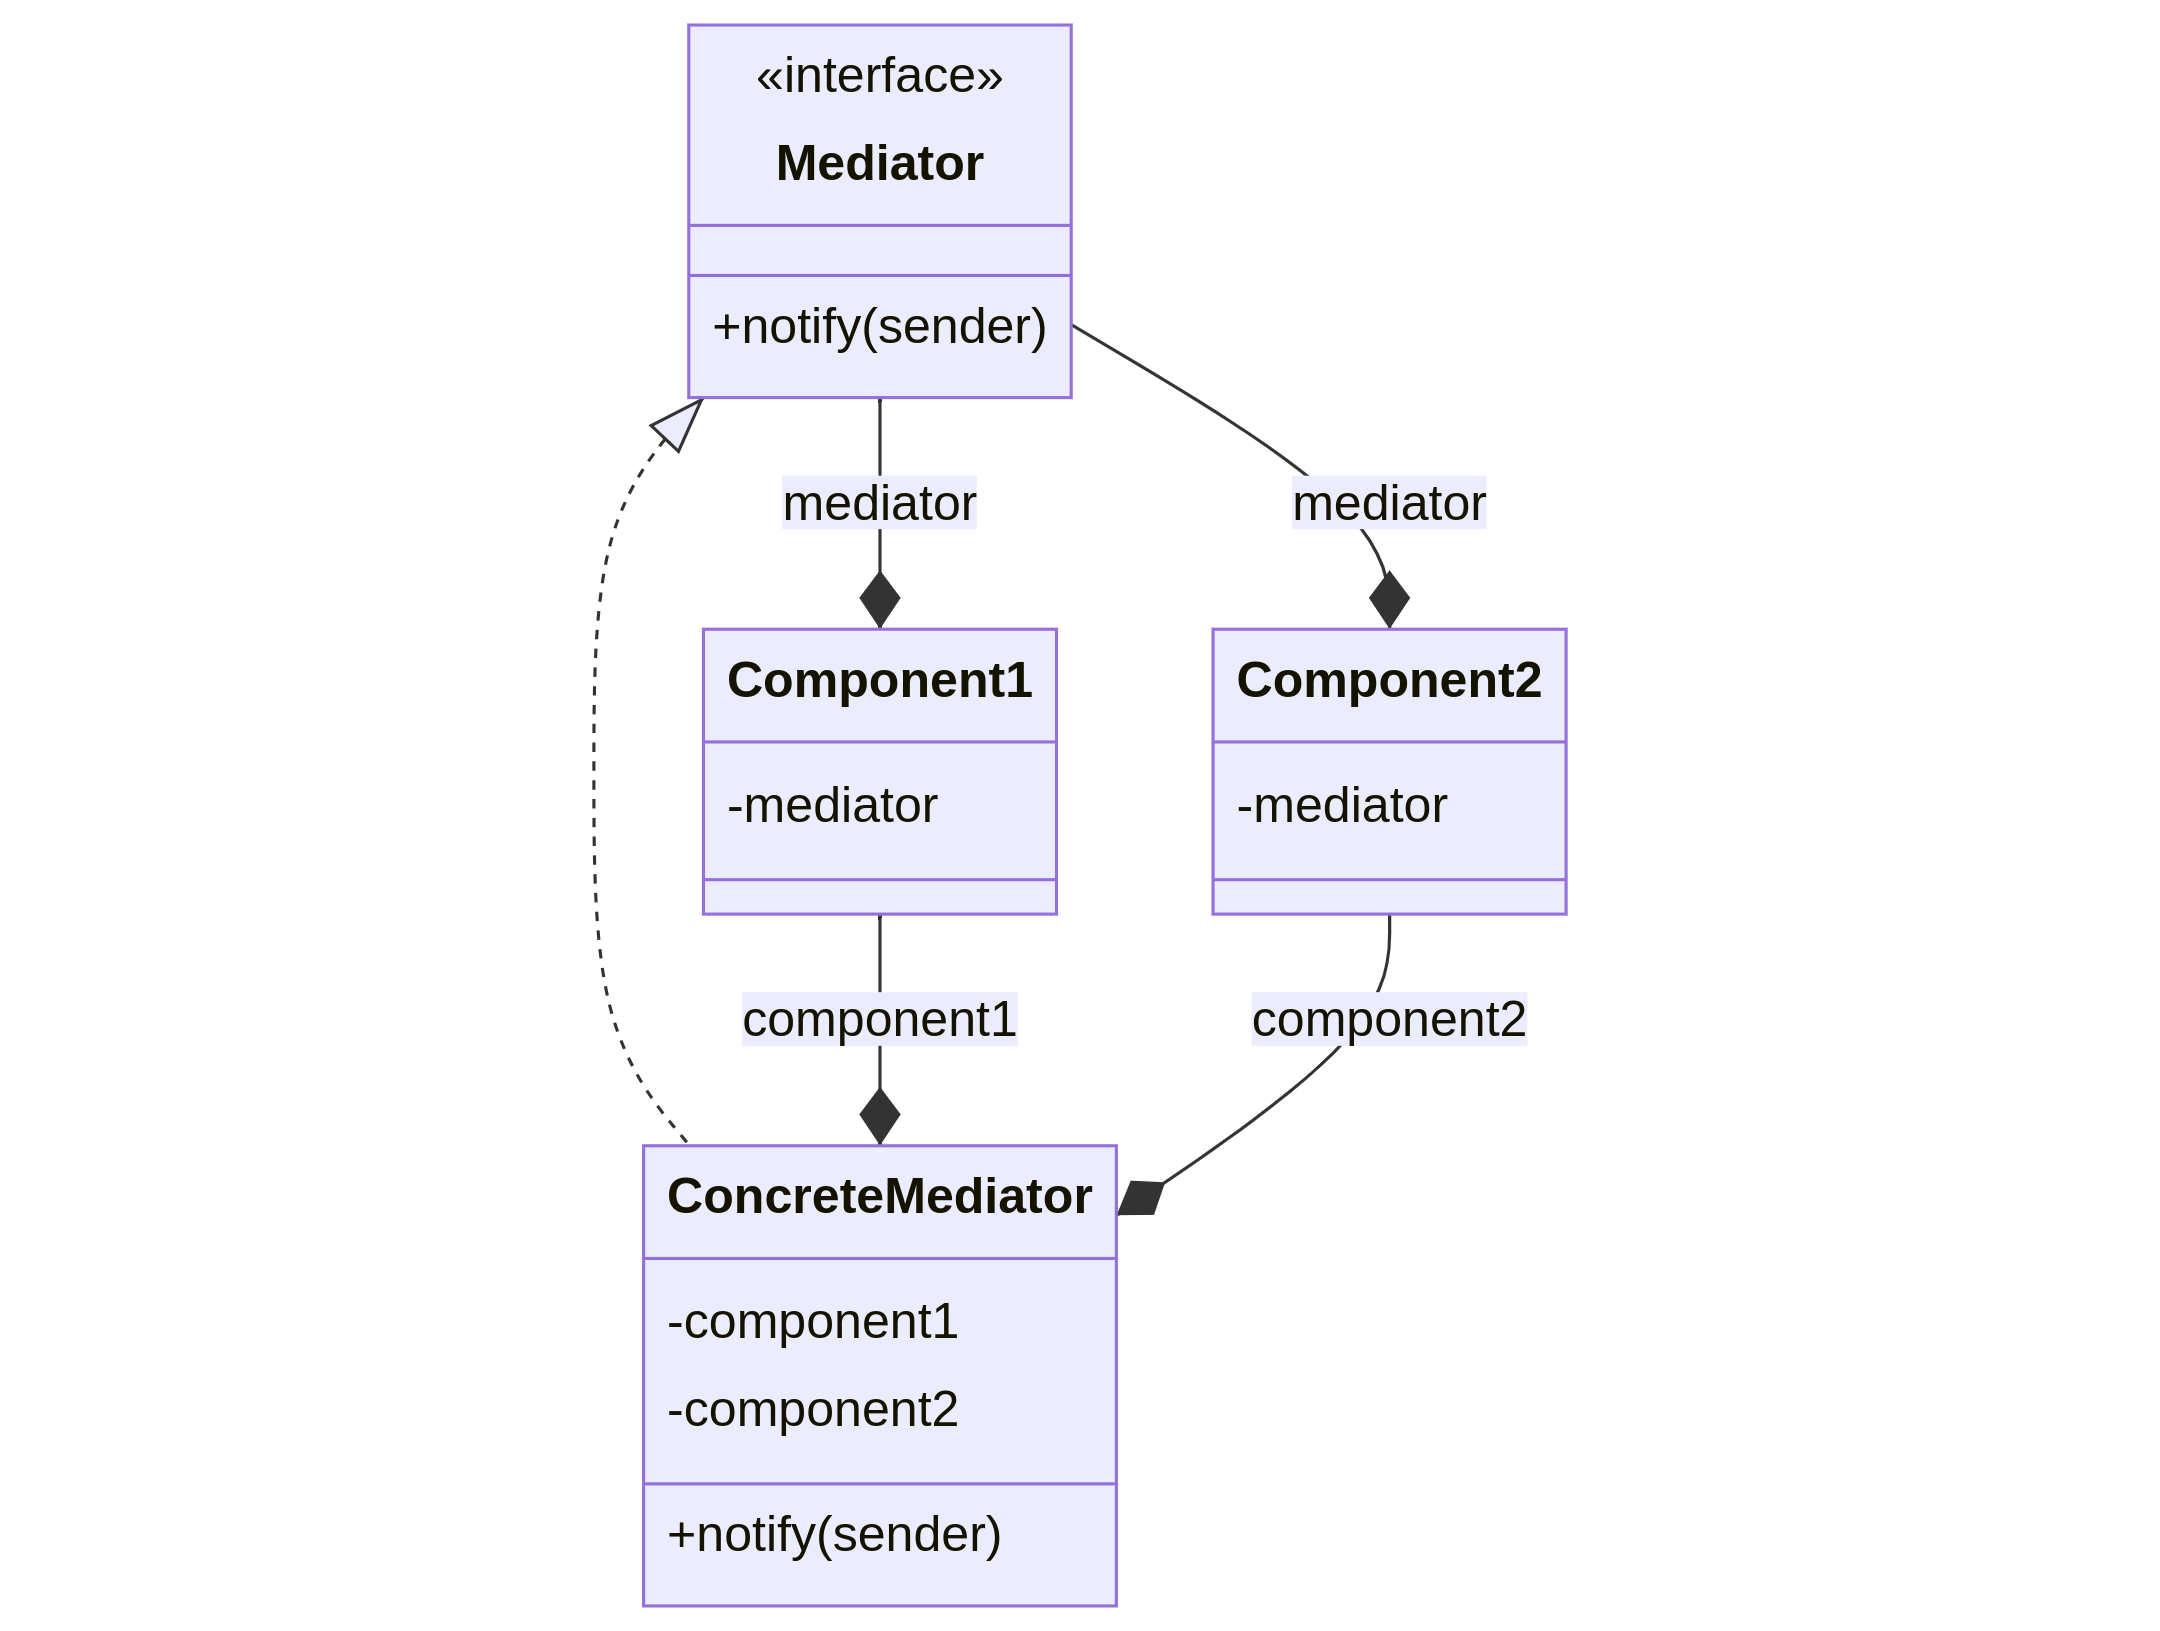
\includegraphics[width=0.75\linewidth]{images/patterns/mediator-class.png}
	\caption{Klassendiagramm Mediator Pattern}
	\label{fig:mediator-class}
\end{figure}

\subsubsection*{Konsequenzen}

Der Mediator kapselt Verhalten, welches ansonsten über mehrere Klassen verteilt wäre. Soll dieses Verhalten spezialisiert werden, so ist nur eine Spezialisierung des Mediators notwendig. Weiterhin verhindert der Mediator eine starke Kopplung der Komponenten. Komponenten- und Mediator-Klassen können bei kompatiblen Interfaces beliebig ausgetauscht werden. Der Mediator vereinfacht außerdem die Multiplizitäten von Objektinteraktionen. Er wandelt $m$:$n$- Beziehungen zwischen Objekten in $1$:$n$-Beziehungen zwischen den Objekten und dem Mediator um. 

Der Mediator bündelt Kontrolle an einem einzigen Punkt. Dies kann zur Übersichtlichkeit beitragen, kann dieser jedoch bei ausreichend komplexer Logik entgegenwirken. Das kann dem Mediator eine monolithische Struktur geben, deren Verhinderung seine eigentliche Aufgabe ist. 

Sind die Abhängigkeiten zwischen den Komponenten zu Komplex, so kann das Observer-Pattern zur Kommunikation zwischen den Komponenten und dem Mediator verwendet werden. Dadurch lassen sich die Abhängigkeiten außerdem flexibler gestalten, sie können also zur Laufzeit einfacher geändert werden.